% document formatting
\documentclass[10pt]{article}
\usepackage[utf8]{inputenc}
\usepackage[left=1in,right=1in,top=1in,bottom=1in]{geometry}
\usepackage[T1]{fontenc}
\usepackage{xcolor}

% math symbols, etc.
\usepackage{amsmath, amsfonts, amssymb, amsthm}

% lists
\usepackage{enumerate}

% images
\usepackage{graphicx} % for images
\usepackage{tikz}

% code blocks
\usepackage{minted, listings} 
\lstset{
  basicstyle=\ttfamily,
  mathescape
}
% verbatim greek
\usepackage{alphabeta}

\graphicspath{{./assets/images}}

\newcommand{\solution}{\textbf{Solution:}} 

\title{COM SCI 132 Week 10}

\author{Aidan Jan}
\date{\today}

\begin{document}
\maketitle

\section*{Advanced Register Allocation}
\subsection*{Chordal vs. Non-chordal graphs}
Remember that register allocation can be written as a graph coloring problem where the color represents registers.\\
\begin{itemize}
    \item t
\end{itemize}
Non-chordal graph:\\
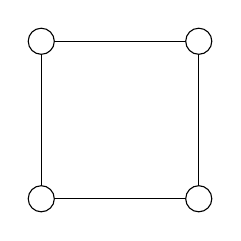
\begin{tikzpicture}
    \node[shape=circle, draw=black] (0) at (0, 0) {};
    \node[shape=circle, draw=black] (1) at (2, 0) {};
    \node[shape=circle, draw=black] (2) at (0, 2) {};
    \node[shape=circle, draw=black] (3) at (2, 2) {};

    \draw [-] (0) -- (1);
    \draw [-] (1) -- (3);
    \draw [-] (3) -- (2);
    \draw [-] (2) -- (0);
\end{tikzpicture}\\
Chordal graphs: (there are no 4(+)-cycles without chords)\\
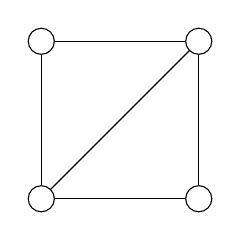
\begin{tikzpicture}
    \node[shape=circle, draw=black] (0) at (0, 0) {};
    \node[shape=circle, draw=black] (1) at (2, 0) {};
    \node[shape=circle, draw=black] (2) at (0, 2) {};
    \node[shape=circle, draw=black] (3) at (2, 2) {};

    \draw [-] (0) -- (1);
    \draw [-] (1) -- (3);
    \draw [-] (3) -- (2);
    \draw [-] (2) -- (0);
    \draw [-] (0) -- (3);
\end{tikzpicture} \hspace{2cm}
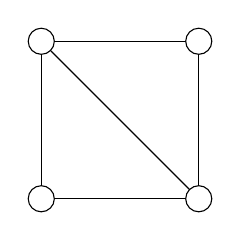
\begin{tikzpicture}
    \node[shape=circle, draw=black] (0) at (0, 0) {};
    \node[shape=circle, draw=black] (1) at (2, 0) {};
    \node[shape=circle, draw=black] (2) at (0, 2) {};
    \node[shape=circle, draw=black] (3) at (2, 2) {};

    \draw [-] (0) -- (1);
    \draw [-] (1) -- (3);
    \draw [-] (3) -- (2);
    \draw [-] (2) -- (0);
    \draw [-] (1) -- (2);
\end{tikzpicture}
\begin{itemize}
    \item about 95\% of interference graphs contain chords.
\end{itemize}

\subsection*{Graph Coloring Complexity}
\begin{tabular}{c | c }
    Type of Graph & Graph Coloring Complexity \\
    \hline
    Interval graphs & polynomial time \\
    $\subseteq$ Chordal graphs & polynomial time \\
    $\subseteq$ General graphs & NP-complete 
\end{tabular}
\begin{itemize}
    \item For chordal and interval graphs, greedy coloring is optimal.
    \item \textbf{Theorem:} A graph $G$ is chorded $\Longleftrightarrow$ $G$ has a simplified elimination order.
    \begin{itemize}
        \item This is good since most register allocation interference graphs are chorded.
    \end{itemize}
\end{itemize}

\subsection*{Example}
Consider the following code:
\begin{verbatim}
    int m(int x, a, d) {    |  x  a  b  c  d  e 
        int b, c            |  |  |        |  
        if (x > 0) {        |  O  O        |
            e = 0           |              |  *
            c = d           |           *  O  |
        } else {            |     *     O     O
            b = 0           |     |  *  
            c = a           |     O  |  *
            e = b           |        O  |     *
        }                   |           |     |
        return e + c        |           O     O
    }
\end{verbatim}

This code generates an interval graph (not chordal), since (a, b, c, e, d) is a 5-cycle without chords.
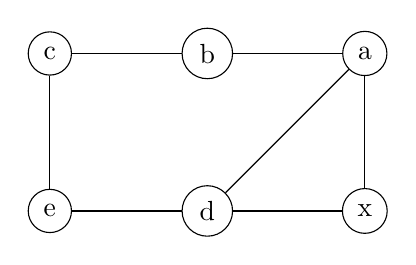
\begin{tikzpicture}
    \node[shape=circle, draw=black] (0) at (0, 0) {e};
    \node[shape=circle, draw=black] (1) at (2, 0) {d};
    \node[shape=circle, draw=black] (2) at (4, 2) {a};
    \node[shape=circle, draw=black] (3) at (2, 2) {b};
    \node[shape=circle, draw=black] (4) at (0, 2) {c};
    \node[shape=circle, draw=black] (5) at (4, 0) {x};

    
    \draw [-] (0) -- (1);
    \draw [-] (1) -- (2);
    \draw [-] (2) -- (3);
    \draw [-] (3) -- (4);
    \draw [-] (4) -- (0);
    \draw [-] (1) -- (5);
    \draw [-] (2) -- (5);
\end{tikzpicture}


\subsection*{Static Single Assignment (SSA)}
This form occurs when two different branches in a program assign to the same variable.  Here are some examples:
\begin{verbatim}

if ___ {            c1, c2 = 0             c1, c2 = 0 
    c = 0           if ___ {               if ___ { 
} else {                c1 = 1                  c1 = 1
    c = 1           } else {                    c = c1
}                       c2 = 1             } else {
__ = c              }                           c2 = 1
                    __ = f(c1, c2)              c = c2
                                           }
                                           __ = c
\end{verbatim}
\begin{verbatim}
    Not SSA Form:       SSA Form:

    x = new B()         x1 = new B()
    x.p(b)              x1.p(b)
    ...                 ...
    x = new C()         x2 = new C()
    x.m(C)              x2.m(C)
\end{verbatim}
\begin{itemize}
    \item GCC and LLVM compile to this form.
\end{itemize}
\pagebreak
\subsection*{Example 2}
\begin{verbatim}
    int m(int x, a, d) {    |  x  a  b  c1 c2 c  d  e1 e2 e 
        int b, c            |  |  |              |
        if (x > 0) {        |  O  O              |
            e1 = 0          |                    |  *
            c1 = d          |           *        O  |
        } else {            |     *     O           O
            b = 0           |     |  *  
            c2 = a          |     O  |     *  
            e2 = b          |        O     |           *
        }                   |              |           |
        e = f(e1, e2)       |           *  |        O  O  *
        c = f(c1, c2)       |           O  O  *           |
        return e + c        |                 O           O
    }
\end{verbatim}
This code generates the following graph:\\
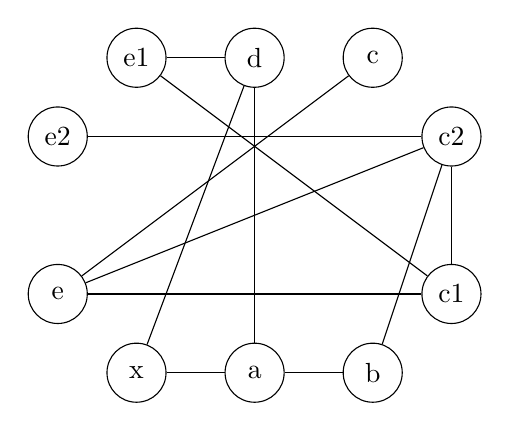
\begin{tikzpicture}
    \node[shape=circle, draw=black, minimum size=0.75cm] (0) at (1, 0) {x };
    \node[shape=circle, draw=black, minimum size=0.75cm] (1) at (2.5, 0) {a };
    \node[shape=circle, draw=black, minimum size=0.75cm] (2) at (4, 0) {b };
    \node[shape=circle, draw=black, minimum size=0.75cm] (3) at (5, 1) {c1};
    \node[shape=circle, draw=black, minimum size=0.75cm] (4) at (5, 3) {c2};
    \node[shape=circle, draw=black, minimum size=0.75cm] (5) at (4, 4) {c };
    \node[shape=circle, draw=black, minimum size=0.75cm] (6) at (2.5, 4) {d };
    \node[shape=circle, draw=black, minimum size=0.75cm] (7) at (1, 4) {e1};
    \node[shape=circle, draw=black, minimum size=0.75cm] (8) at (0, 3) {e2};
    \node[shape=circle, draw=black, minimum size=0.75cm] (9) at (0, 1) {e };

    \draw [-] (0) -- (1); 
    \draw [-] (0) -- (6); 
    \draw [-] (1) -- (6); 
    \draw [-] (6) -- (7);
    \draw [-] (7) -- (3);  
    \draw [-] (1) -- (2);  
    \draw [-] (2) -- (4);  
    \draw [-] (4) -- (8);  
    \draw [-] (4) -- (3);  
    \draw [-] (9) -- (3);  
    \draw [-] (4) -- (9);  
    \draw [-] (5) -- (9);  

\end{tikzpicture}
(This is a chordal graph.)
\subsection*{Spilling}
\begin{itemize}
    \item Spilling is NP-complete even for chordal graphs
\end{itemize}
Compiler:
\begin{center}
    Source $\longrightarrow$ SSA $\longrightarrow$ RISC-V\\
    $\uparrow$\\
    Optimal register allocation in polynomial time
\end{center}
(We can't have optimal register allocation and optimal spilling in polynomial time)

\subsection*{Graphs}

\begin{center}
    Interval Graphs $\subseteq$ Chordal Graphs $\subseteq$ All undirected graphs
\end{center}
\begin{itemize}
    \item 100\% of procedures \textbf{in SSA form} have chordal interference graphs
    \item 95\% of procedures have chorded interference graphs
    \item All of the procedures are possible as interference graphs
\end{itemize}

\pagebreak
\subsection*{Parallel Assignment}
Consider Example 2.
Instead of writing
\begin{verbatim}
    e = f(e1, e2)
    c = f(c1, c2)
\end{verbatim}
write
\begin{verbatim}
    c, e = f(c1, c2), f(e1, e2)
\end{verbatim}
This actually \textit{reduces} the complexity because by doing this, \texttt{e} and \texttt{c1, c2} no longer exist at the same time.
\end{document}